\chapter{Introduction to cryptography} % Main chapter title
\label{ch:intro_crypto}

%----------------------------------------------------------------------------------------

\section{About security}
A stated in chapter \ref{chap:bc}, \textbf{information security} is not easy to define. Even the National Institute for Science and Technology (NIST, the main American institute for standards of connected systems) periodically changes its definition of security, showing how we switched from a computer-centric to an information-centric kind of security:

\begin{itemize}
    \item \textbf{Computer Security}: the protection afforded to an automated information system in order to attain the applicable objectives of preserving the integrity, availability and confidentiality of information system resources (includes hardware, software, firmware, information/data, and telecommunications)\footnote{NIST, October 1995, \url{https://doi.org/10.6028/NIST.SP.800-12}}.
    \item \textbf{Information Security}: the protection of information and information systems from unauthorized access, use, disclosure, disruption, modification, or destruction in order to ensure confidentiality, integrity, and availability\footnote{NIST, June 2017, \url{https://doi.org/10.6028/NIST.SP.800-12r1}}.
\end{itemize}

The ultimate goal thus is not to protect the computer, but the most important asset: data. The main aspects of security can be summarised in six concepts or policies, all of them strongly tied together: we cannot ensure confidentiality without authentication, integrity without access control, etc.:

\begin{enumerate}
    \item \textbf{access control};
    \item \textbf{authentication};
    \item \textbf{availability};
    \item \textbf{confidentiality};
    \item \textbf{integrity};
    \item \textbf{non repudiation}.
\end{enumerate}

In general, information security:
\begin{itemize}
    \item supports the mission of the organization;
    \item represents an integral element of sound management;
    \item implements protections so as to be commensurate with risk;
    \item makes roles and responsibilities explicit;
    \item pushes responsibilities for system owners beyond their own organization;
    \item requires a comprehensive and integrated approach;
    \item is assessed and monitored regularly;
    \item is constrained by societal and cultural factors.
\end{itemize}

%-------------------------------------------

\subsection{Access control}
\textbf{Access control} is the security technique that regulates who or what can view, use or access a place or other resources. It is strongly coupled with authentication, since it first assigns profiles to users, then limits service access to authorized profiles only. This technique consists of many rules that are not easy to define, and which require careful consideration. As one could imagine, to perform access control accounting techniques are used.

It is interesting noting that after a security violation, access control is the first policy to be examined. The network manager is the first person under investigation: he/she must prove that is not responsible for the attack, since it could have potentially serious legal consequences.

%-------------------------------------------

\subsection{Authentication}
\textbf{Authentication} is the process of verifying whether someone (or something) is, in fact, who (or what) it has declared to be: sometimes attackers might be posing as someone else in order to obtain reserved information meant for another person or device only.

Digital signature functions are used in order to obtain authentication.

%-------------------------------------------

\subsection{Availability}
\textbf{Availability} provides an assurance that the system and data (the overall service) can be accessed by and fulfill the requests of authorized users, whenever and wherever they are needed.

Service availability is the most difficult quality to guarantee, as it requires accurate network planning; for example, it is not achieved if a Denial of Service (DOS) attack is ongoing (in this case, our mission would be to make it so that realizing a DoS attack would be onerous for an attacker).

Note that periodically checking a system's availability is not an effective method for ensuring this policy, because an attacker could put the system down and bring it back up between two checks.

%-------------------------------------------

\subsection{Confidentiality}
\textbf{Confidentiality} is the security technique that protects information from being accessed by unauthorized parties. The exchanged data must remain \textbf{secret} between sender and receiver.

Normally, confidentiality is achieved by using cryptography algorithms, since networks allow for sniffing packets and non-encrypted data could potentially be read by someone else.

%-------------------------------------------

\subsection{Integrity}
\textbf{Integrity} is the assurance that the information is trustworthy and accurate. Data thus must reach destination without having been altered, either while being transmitted or stored. Usually data integrity is achieved by using hash functions.

Note that encrypted data does not ensure integrity, because sometimes cryptographic methods are vulnerable to attacks, and cryptographed data can be changed nonetheless (e.g. through a bit flipping attack). Also, there can be integrity without confidentiality.

%-------------------------------------------

\subsection{Non repudiation}
\textbf{Non repudiation} is the assurance that someone cannot deny the validity of something. It is a very important policy when documents are exchanged, and it is usually achieved with digital signature functions.

Digital signatures are a lot stronger than regular signatures\footnote{The human version of non repudiation, even though not very obvious, is quite funny. Consider signing a letter: even though we were the ones who signed it, we can always say that it was not our signature, and that someone else forged it. Nobody can claim that we are lying, because we ourselves are the ultimate authority that can say if a certain signature is ours and/or if we signed the letter. Only a graphological test (which, in fact, consists of another person analysing the signature - making all this rather paradoxical) could check if the signature has really been forged, but it is a long and painful process that is normally not undertaken.}. However, they are cryptographic methods, so they will be valid only for a number of years; after a certain deadline expires they are not valid anymore, meaning that anyone could claim anything about documents signed with an expired digital signature.

%----------------------------------------------------------------------------------------

\section{Cryptography principles}
\textbf{Cryptography} is the basis to do non repudiation (digital signatures), access control (because it is based on authentication, which in turn is based on digital signatures), integrity and confidentiality - basically everything but availability.

Cryptography is as old as the world; it means "to write something in an obscure way", and it describes how to exchange information in a way that only source and destination can understand.

In general, every message sent from a source to a destination contains information that can be quantified\footnote{If something contains information, then it cannot be random -  otherwise it would have no information.}. The point of cryptography is to hide this information to the point that an attacker cannot distinguish between meaningful data and random, uncorrelated noise (such as white noise). This is called \textbf{perfect secrecy}. Is it achievable? Yes, but actually no - and we are going to see why.

\vspace{0.2em}

\textbf{Note}: We must never invent our own cryptographic algorithm, because we will most certainly fail: it is a very hard mathematical task for which reinventing the wheel does not work (at all).

%-------------------------------------------

\subsection{Hash functions}
A \textbf{hash function} is a mathematical function that takes an input (in our case, a message) and outputs a \textbf{digest}, which is a \textit{smaller} piece of data of fixed dimension $n$ that has some mathematical properties (see fig. \ref{fig:hash}). Generally speaking, any minimal change to the input made by the hash function will provide a completely different result in the digest.

Hash functions are commonly used to resolve integrity guarantee of transmitted documents; they are realized with elementary operations such as \textbf{shift} and \textbf{XOR}, so they are computationally very fast.

\begin{figure}[H]
\centering
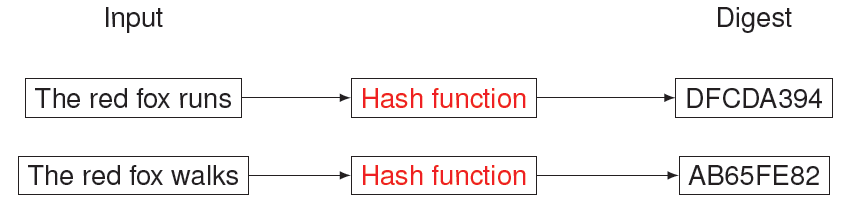
\includegraphics[scale=0.5]{img/hash.png}
\decoRule
\caption{An example of how hash functions work.}
\label{fig:hash}
\end{figure}

A hash function can and must be defined in terms of mathematical properties, because these are useful for a number of reasons. For example, if a person A (the sender) sends a message (some data) and its digest to another person B (the receiver), B can calculate the message's digest by using the same hash function as A (which is already known to both) and compare it with the one received from A, as shown in fig. \ref{fig:hashAB}. If the two digests are the same, then the message received from A has not been modified; otherwise, someone might have intentionally edited the data during transmission, and integrity has been lost.

\begin{figure}[H]
\centering
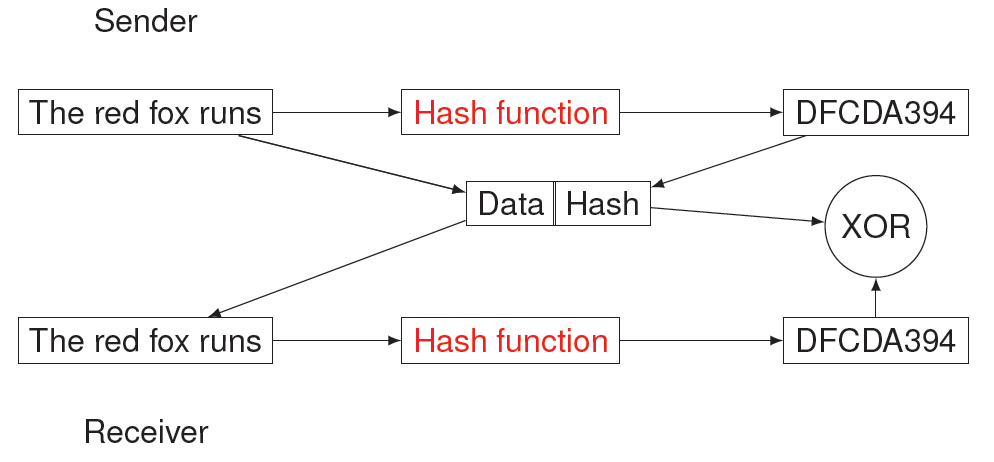
\includegraphics[scale=0.4]{img/hash_AB.png}
\decoRule
\caption{An example of how a digest can be useful to verify the integrity of a message. Note that, unlike this diagram, in real life we never want to send the message and its digest through the same channel, because an attacker could modify both and thus fool the receiver into thinking that the data has not been altered. Forcing an attacker to break two different channels represents an additional step in difficulty and security.}
\label{fig:hashAB}
\end{figure}

%----------------------

\subsubsection{Properties of hash functions}
In mathematical terms, a \textbf{hash function} is a function $H : X \rightarrow Y$ which maps an input $m$ of arbitrary finite length to an output $y = H(m)$ of fixed length $n$ (\textbf{ease of computation}). Domain $X$ contains all possibles messages, while codomain $Y$ all possibles digests; being $n$ of arbitrarily fixed length, $Y$ will be much smaller than $X$: $dim(X) \ll dim(Y)$ (\textbf{compression}).

Let us suppose that an attacker knows the digest of a message, but not the function that generated it. We should not be able to find another message that has the same hash - not because it is \textit{impossible}\footnote{\textbf{Impossible} means that a task cannot be performed, not even by brute force (i.e. trying every possible combination of bytes or secrets from a list, knowing the secret's length - an attack that is always possible).}, but because it is \textit{infeasible}\footnote{\textbf{Infeasible} means that a task cannot be performed within a reasonable amount of time with a reasonable amount of computational power.}. This property is called \textbf{pre-image resistance}, and it basically means that an attacker cannot pretend to be a legitimate user and send a message with a certain hash in order to later claim that the message was different (invalidating the original message).

\vspace{0.2em}

In short, the main properties of a hash function are:

\begin{enumerate}
    \item \textbf{compression}: $H : X \rightarrow Y$, with $dim(X) \ll dim(Y)$;
    \item \textbf{ease of computation}: given $H$ and an input $m$, $y = H(m)$ is very ease to compute;
    \item \textbf{pre-image resistance}: given a hash value $h$, it is computationally \textit{infeasible} to find any message $m$ such that $H(m) = h$;
    \item \textbf{2\textsuperscript{nd} pre-image resistance}: given a message $m$, it is computationally \textit{infeasible} to find any message $m'$ such that $H(m') = H(m)$;
    \item \textbf{collision resistance}: it is computationally infeasible to find any two distinct, arbitrarily chosen inputs $m$ and $m'$ such that $H(m') = H(m)$. This is the most difficult property to achieve in practice; note that having a hash function resistant to collision does not mean that it also has \textbf{pre-image resistance} and \textbf{2\textsuperscript{nd} pre-image resistance}.
\end{enumerate}

If a hash function does not respect even one of these properties, it cannot be used for cryptography purposes. However, not all of them are easy to achieve, nor can they be mathematically proven for an algorithm.

%-------------------------------------------

\subsection{HMAC}
We saw that hash functions are useful to guarantee integrity. What about authentication? For this task we need a \textbf{Hash Message Authentication Code}, or \textbf{HMAC}, which combines a hash function with a secret key.

The most used HMAC algorithm is the one from RFC 2104\footnote{\url{https://tools.ietf.org/pdf/rfc2104.pdf}}, which consists of the application of the hash function $H$ to a message $m$ and a shared secret key $K$ using equation \ref{eq:hmac} in order to obtain a digest in output:

\begin{equation}
\label{eq:hmac}
    \mathit{HMAC}(K,m) = H\Big((K' \oplus opad) \parallel H (K' \oplus ipad) \parallel m\Big)
\end{equation}
where

\begin{itemize}
    \item $H$ is a cryptographic hash function;
    \item $m$ is the message to be authenticated, divided into blocks of size $j$ (with $j$ depending on the hash function used);
    \item $K$ is the secret key;
    \item $K'$ is a block-sized key derived from the secret key $K$ either by padding to the right with zeros up to the block size, or by hashing down to less than or equal to the block size first and then padding to the right with zeros:
    
    \begin{equation}
        K' = \begin{cases}
        K &\text{if $dim(K) = j$}\\
        K \parallel pad(0) &\text{if $dim(K) < j$}\\
        H(K) &\text{if $dim(K) > j$}\\
        \end{cases}
    \end{equation}
    
    \item $\parallel$ denotes concatenation;
    \item $\oplus$ denotes bitwise exclusive-or (XOR);
    \item $opad$\footnote{\label{foot:pad}The values of $opad$ and $ipad$ are not critical to the security of the algorithm, but are defined in such a way to have a large Hamming distance from each other, and so the inner and outer keys will have fewer bits in common.} is the block-sized outer padding, consisting of bytes valued 0x5c repeated $\frac{j}{8}$ times;
    \item $ipad$\footref{foot:pad} is the block-sized inner padding, consisting of bytes valued 0x36 repeated $\frac{j}{8}$ times.
\end{itemize}

The secret key is first used to derive two keys – inner and outer; the first pass of the algorithm produces an internal hash derived from the message and the inner key, while the second pass produces the final HMAC code derived from the inner hash result and the outer key. 

It is worth noting that the final result will depend not only on the message, but also on the key, meaning that even if the attacker has the message he/she might not be able to decrypt it. $K$ should be large and random enough in order to not contain predictable bits, because otherwise an attacker could it find by using a brute force attack. If $K$ is shorter than $j$  bits we pad $K$ with a $0$ padding and then we either use it as it is, or we hash it and add a maximum entropy\footnote{\textbf{Entropy} is a measure of the informative content of a message. A message with maximum entropy is made entirely out of random bits (does not contain information).} number.

%----------------------

\subsubsection{HMAC in practice}
The digest can be calculated if and only if \textit{both} participants know the key $K$, so we will need authentication in order to ensure that they really are who they claim to be (and thus avoid giving the key to a potential attacker).

Suppose that A sends $m$ and $\mathit{HMAC}(K, m)$ to B in the same packet: if an attacker E intercepts both informations, he/she cannot recalculate $\mathit{HMAC}(K, m)$ because he/she does not know the key $K$, but he/she can easily modify $m$ in $m'$.

It is then clear that the main problems of HMAC are:

\begin{enumerate}
    \item finding a \textbf{secure way to exchange $K$} (and no, Internet is not the answer);
    \item \textbf{brute force attacks}: E could intercept a packet and try to predict $K$. This type of
attack is computationally infeasible, \textit{but} if the key is derived from a password, E can perform a dictionary
attack, since generating words in a dictionary takes only a few minutes. This issue is more common than one might think.
\end{enumerate}

%----------------------

\subsubsection{Final considerations}
HMAC does not state the hash function to be used, so we must choose the most appropriate one. We must be aware of the vulnerabilities that from time to time are found in hash functions and eventually change it, since the more they are used, the more they are studied and more vulnerabilities are found. For example, we should use \textbf{SHA3} instead of SHA2 or SHA1 (which are actually still widely used despite being severely broken).

If we use a weak hash function, an attacker could forge a message that would be considered by the receiver as valid; this is a very bad case, because the attacker could not just send false messages, but also find the secret key.

%-------------------------------------------

\subsection{Symmetric key encryption}
Symmetric key algorithms are algorithms for cryptography that use the same cryptographic keys for both encryption of plaintext (the original message) and decryption of ciphertext (the encoded message), as depicted in fig. \ref{fig:symm}. The keys, in practice, represent a shared secret between two or more parties that can be used to maintain a private information link.

Algorithms used for encryption and decryption can either be symmetrical or asymmetrical.

\begin{figure}[H]
\centering
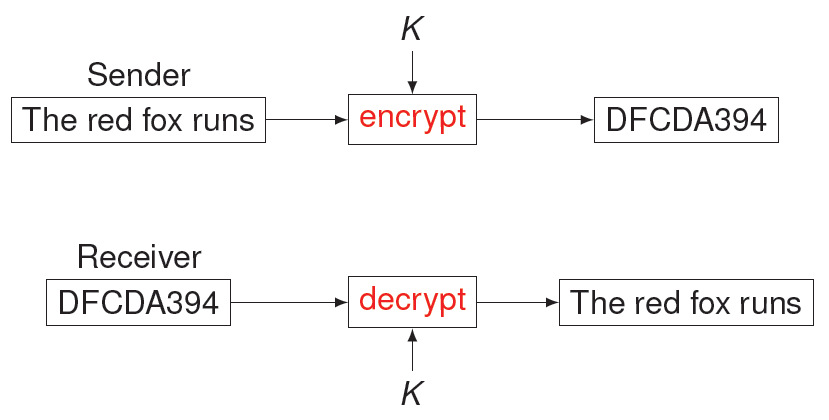
\includegraphics[scale=0.45]{img/symm.png}
\decoRule
\caption{Symmetric key encryption and decryption.}
\label{fig:symm}
\end{figure}

%----------------------

\subsubsection{Symmetric key encryption limitations}
The requirement that both parties have access to the secret key is one of the main drawbacks of symmetric key encryption, in comparison to public key encryption (also known as asymmetric key encryption).

Everything works if and only if we can ensure that nobody except for the sender and the receiver knows the keys. This statement is extremely weak: we can never assume it to be true, because the sender or the receiver could have been compromised, or the receiver is untrusted, and/or we cannot exchange different keys on the fly. In other words, symmetric key encryption is blind: it does not tell us anything about the identity of the sender, nor if the message has been modified or not.

%----------------------

\subsubsection{Use with HMAC}
In order to ensure the integrity of a message in symmetric key encryption, we can use it combined with HMAC in the following way:

\begin{enumerate}
    \item generate an HMAC with a secret key $K$;
    \item encrypt the whole message (HMAC included) with another secret key $K'$;
    \item by comparing the message and its HMAC, the receiver can tell if everything is right (or not).
\end{enumerate}

We use HMAC instead of a simple hash because if we used a hash and the attacker would recover the outer key $K'$ (the one used for symmetric encryption), he/she could change the message and its hash - so key $K'$ is an increased step in security.

Note that in spite of this method, the problems of privately sending the keys and ensuring the sender's identity remain.

%-------------------------------------------

\subsection{Asymmetric key encryption}
\textbf{Asymmetric key encryption} does not use a shared key; instead, both participants (which we name A and B) have two keys:

\begin{itemize}
    \item a \textbf{private key} $Pri_A$, $Pri_B$
    \item a \textbf{public key} $Pub_A$, $Pub_B$
\end{itemize}

Like their name implies, private keys must be kept secret: only A knows $Pri_A$ and only B knows $Pri_B$. Public keys can instead be disseminated anywhere, because they do not need to be protected; both A and B know $Pub_A$ and $Pub_B$, as well as possibly many other people. Obviously, for any person X, it must be computationally infeasible to obtain $Pri_X$ through $Pub_X$ and vice versa.

In an asymmetric key encryption scheme, anyone can encrypt messages using the public key, but only the holder of the paired private key can decrypt them.  An attacker could recover the message that has been sent, but because he/she does not know the private key, he/she will not be able to decrypt it. Thus, asymmetric key encryption works as follows (fig. \ref{fig:asymm}):

\begin{enumerate}
    \item sender (A) uses the receiver's (B) public key $Pub_B$ to encrypt his or her message $m$, obtaining $m'$;
    \item B uses his or her private key $Pri_B$ to decrypt $m'$.
\end{enumerate}

\begin{figure}[H]
\centering
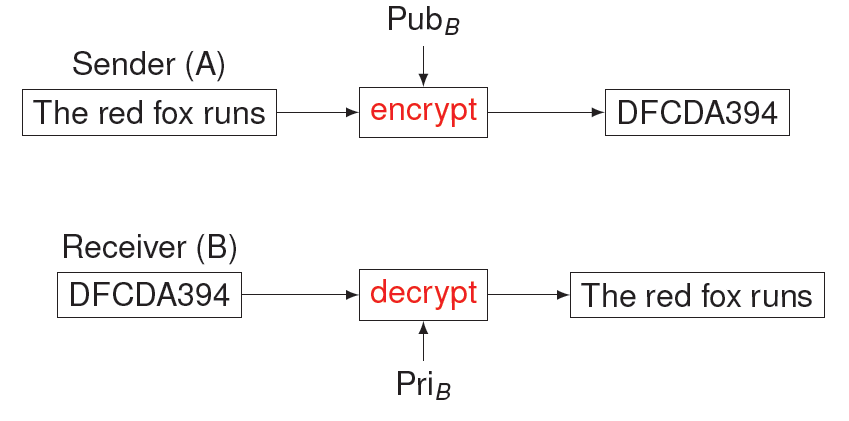
\includegraphics[scale=0.5]{img/asymmkey.png}
\decoRule
\caption{Asymmetric key encryption and decryption.}
\label{fig:asymm}
\end{figure}

The algorithm for encryption and decryption is the same for both operations: if we use the algorithm with one key we obtain a message that can be reverted to the original one by going through the algorithm with the second key (in other words, the second key decrypts the data encrypted by the first one).

Keys are usually joint generated with specific programs, like \textit{ssh-keygen} in Linux environments. It is not necessary to agree in advance on a common encryption/decryption key; an unpredictable (typically large and random) number is used to begin generation of an acceptable pair of keys suitable for use by an asymmetric key algorithm.

%----------------------

\subsubsection{Asymmetric key encryption: pros and cons}
The overall security of this method depends entirely on the \textbf{secrecy of the private key}: if we trust that the private key has been kept private by somebody or something, then whenever we get a message that can be decrypted by the public key paired with that specific private key, we know for sure that the only entity able to encrypt that message was the real sender. 

It is worth noting that in this way we guarantee \textbf{confidentiality}, and solve the problem of identity.

%-------------------------------------------

\subsection{Digital signature}
\textbf{Digital signature} is based on asymmetric key encryption, and in fact uses the same principles, only inverted: since in this case we do not care about confidentiality, but only want to \textbf{ensure the identity} (\textbf{non repudiation}) of the sender, we use A's private key $Pri_A$ to encrypt $m$. This way everybody will be able to decrypt the message with A's public key $Pub_A$, but we will guarantee that the sender was really A (the message has been \textbf{signed} by A, fig. \ref{fig:ds}).

\begin{figure}[H]
\centering
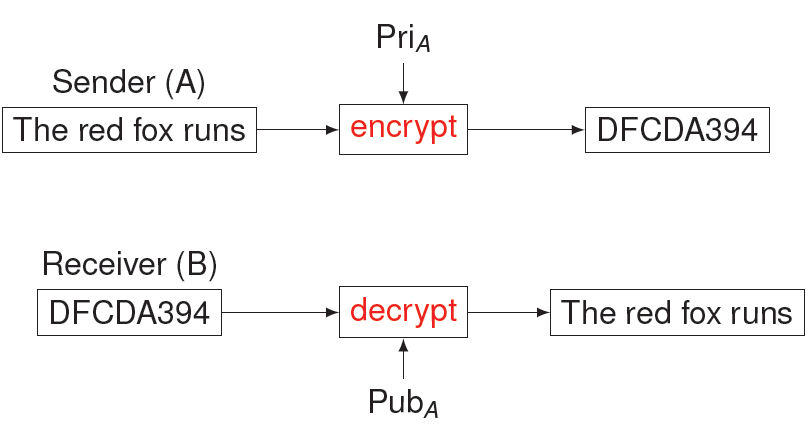
\includegraphics[scale=0.5]{img/ds.png}
\decoRule
\caption{Digital signature example.}
\label{fig:ds}
\end{figure}

%-------------------------------------------

\subsection{Mixed key encryption}
In day-to-day life neither purely symmetric nor purely asymmetric key encryption is used, but instead algorithms which combine these two methods in creative ways have been devised in order to obtain better security.

\begin{figure}[H]
\centering
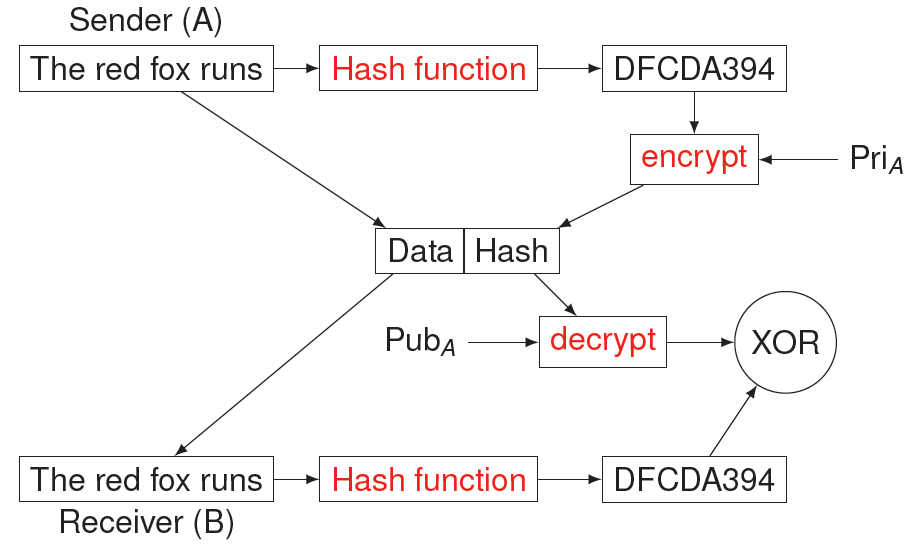
\includegraphics[scale=0.5]{img/mix.png}
\decoRule
\caption{An example of mixed symmetric and asymmetric key encryption.}
\label{fig:mix}
\end{figure}

The most common way of doing this is to encrypt a symmetric key with an asymmetric key. We use asymmetric cryptography to set up the communication, i.e. to negotiate a secret \textbf{session key} that is going to be used during that session. At this point the secret is known only by the sender and the receiver, and can be safely used to exchange private messages between them, ensuring confidentiality, integrity and identification.

Like its name implies, a session key is only valid during the communication session that it has been created for; new sessions will have to generate new secret keys.

%----------------------

\subsubsection{Multiple senders/receivers}
In cases like group chats where multiple ($n$) senders/receivers exist we must use a shared secret key in order to avoid computationally inefficient or even infeasible communication algorithms. However, this is a whole different problem which we do not discuss here; it is complicated by many additional factors, such as ensuring that someone banned out of the chatroom cannot return until not re-authenticated - while maintaining communication active for everyone else.